\documentclass[11pt,a4paper]{article}
\usepackage[T1]{fontenc}
\usepackage[utf8]{inputenc}
\usepackage{lmodern}
\usepackage[margin=20mm]{geometry}
\usepackage{amsmath,graphicx,float}
\usepackage[font=small,labelfont=bf]{caption}
\usepackage[hidelinks]{hyperref}
\graphicspath{{../figures/}}
\setlength{\parindent}{0pt}
\setlength{\parskip}{4pt}
\setlength{\textfloatsep}{10pt}
\setlength{\intextsep}{8pt}
\begin{document}
\begin{center}
{\Large\bfseries DT081A -- Signal and Image Processing\par}
{\large Laboratory 1 Report\par}
Sections 1.1--1.3 -- Signals, Fourier Analysis and Sampling\par
Jakob Obid\par
4 November 2026
\end{center}

\section{Introduction}
This part of Lab 1 compares sine, square and sawtooth waves.
It shows how frequency and addition change a signal.
FFTs were also used to study fixed frequencies, noise and a chirp.
I also tested how different sampling rates affect a signal.

\section{Experimental Setup}
NumPy and Matplotlib were used. All signals use the teacher's time vector,
\texttt{t = np.linspace(0, 1, 1000)}: 1,000 points from 0 to 1 second,
including both ends. The starting signals are a 10 Hz sine and a 5 Hz square.
Their amplitudes were kept unchanged.
For Section 1.2, the original 10 Hz and 20 Hz sines have amplitudes 1 and 0.5.
The FFT uses the time step between the given points.
I used the teacher's sampling examples and tested a 23 Hz sine wave sampled at 8 Hz.

\section{Results and Analysis}
\subsection{Signal Generation and Visualization}

\subsubsection*{Q1. Modify the code to create a sawtooth wave. Describe the mathematical function you used.}
\textbf{Answer:} The function is
\(s(t)=2(5t-\lfloor5t\rfloor)-1\).
Here, \(\lfloor5t\rfloor\) means rounding down to a whole number.
Subtracting it leaves the part of a cycle between 0 and 1.
Scaling by 2 and subtracting 1 gives a rising ramp from $-1$ towards $+1$.
It jumps back every 0.2 seconds, so its frequency is 5 Hz (Figure~\ref{fig:sawtooth}).

\begin{figure}[H]
\centering
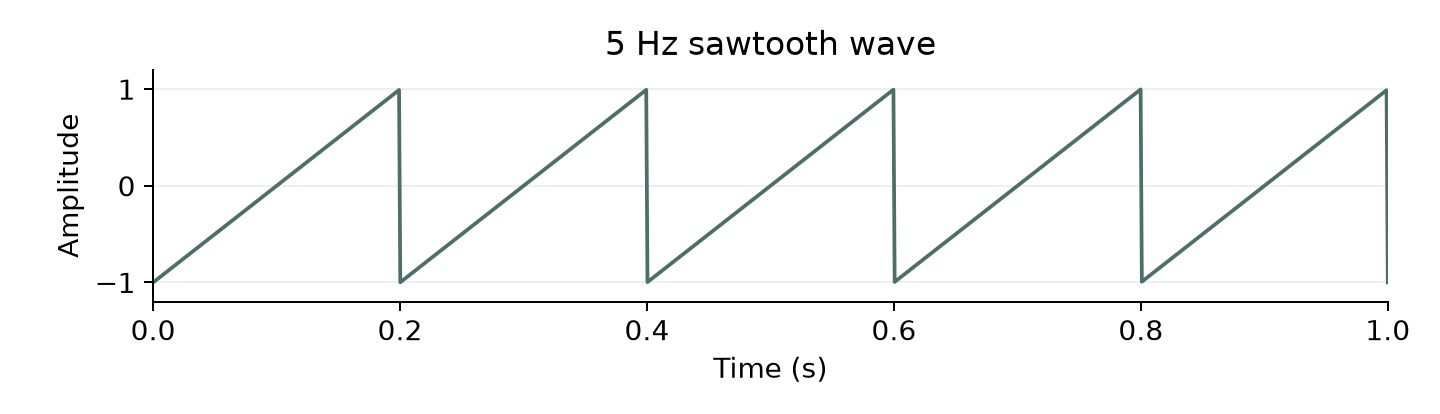
\includegraphics[width=0.88\linewidth]{q1_sawtooth.png}
\caption{Five rising ramps during one second. Each ramp ends with a jump back.}
\label{fig:sawtooth}
\end{figure}

\subsubsection*{Q2. Change the frequency of the sine wave to 20 Hz. How does this affect the plot?}
\textbf{Answer:} The 20 Hz sine has 20 cycles in one second instead of 10.
The waves are closer together in time. The amplitude stays the same (Figure~\ref{fig:sines}).

\begin{figure}[H]
\centering
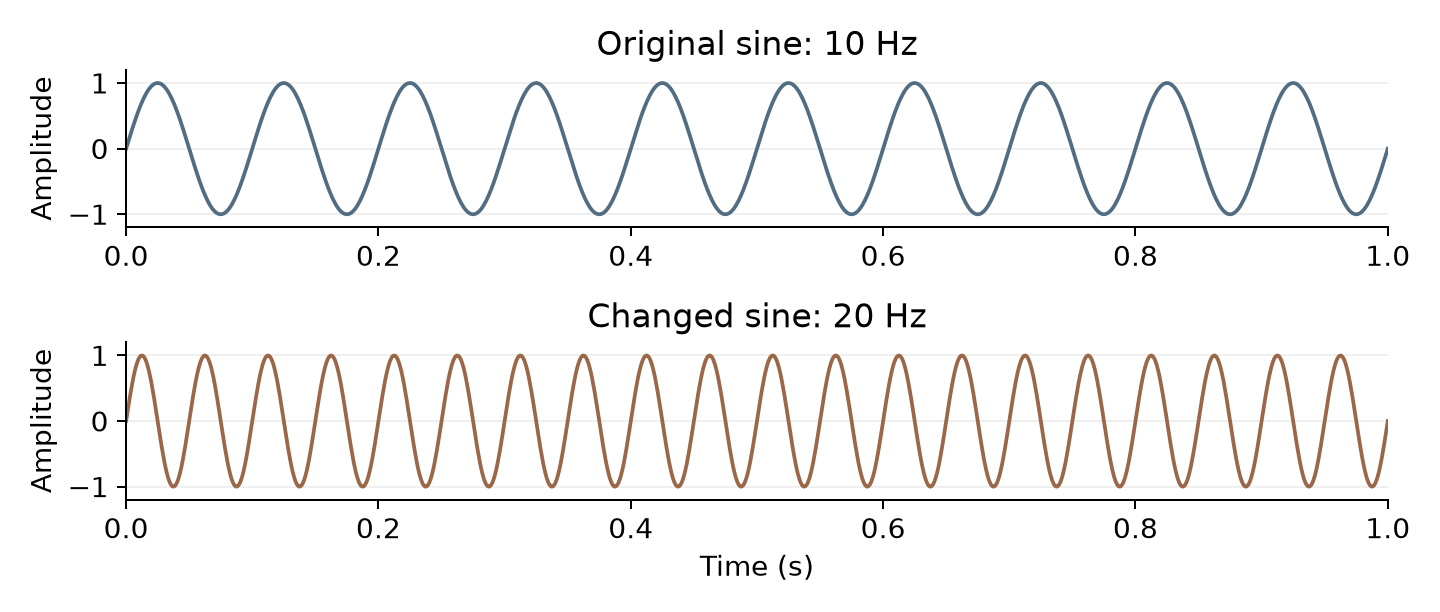
\includegraphics[width=0.88\linewidth]{q2_sine_frequencies.png}
\caption{The same one-second interval and amplitude limits show twice as many cycles at 20 Hz.}
\label{fig:sines}
\end{figure}

\subsubsection*{Q3. What happens to the square wave if you change the sign function to \texttt{np.ceil(np.sin(2 * np.pi * 5 * t)) * 2 - 1}? Explain why.}
\textbf{Answer:} The two expressions give the same value at 999 of the 1,000 samples.
Only the first sample differs: at $t=0$, \texttt{np.sign()} gives 0,
while the replacement gives $-1$.

For a positive sine value, rounding up gives 1, so the replacement gives $+1$.
For a negative value strictly between $-1$ and 0, rounding up gives 0,
so the result is $-1$. At zero, it also gives $-1$, while \texttt{np.sign(0)} gives 0.
If the sine is exactly $-1$, the replacement gives $2(-1)-1=-3$.
No sampled sine value was exactly $-1$, so $-3$ did not appear in these results.

\subsubsection*{Q4. Create a composite signal by adding the sine wave and square wave together. Plot this new signal and describe its characteristics.}
\textbf{Answer:} The original 10 Hz sine was added to the 5 Hz square.
The sine gives the curved parts, and the square gives sudden jumps.
The sampled values range from about $-2$ to $+2$ (Figure~\ref{fig:composite}).

\begin{figure}[H]
\centering
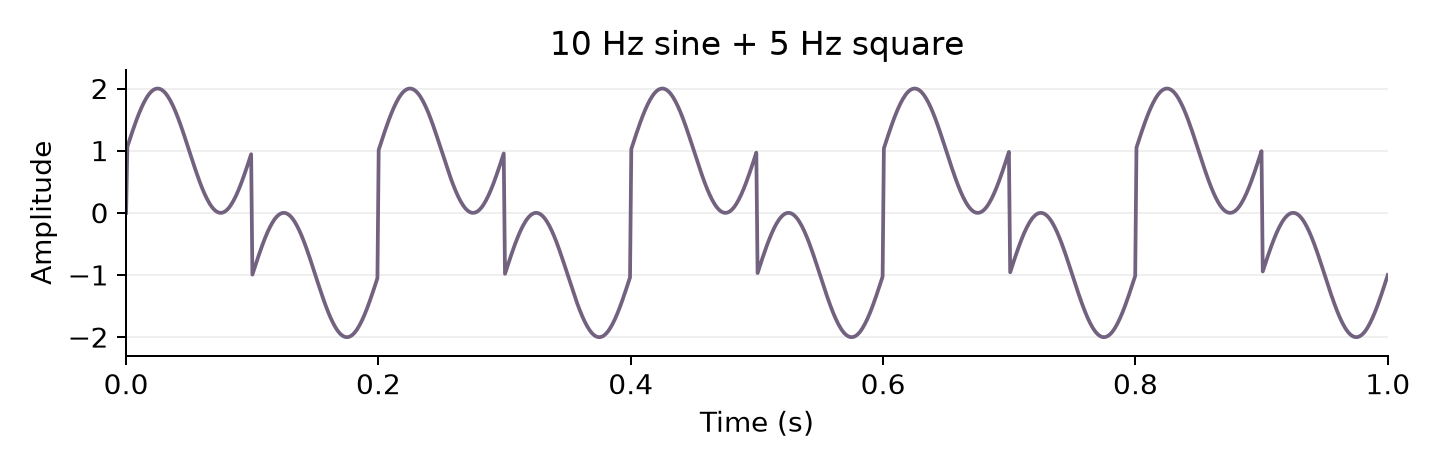
\includegraphics[width=0.92\linewidth]{q4_composite.png}
\caption{The original sine and square added together, without changing their amplitudes.}
\label{fig:composite}
\end{figure}

\subsubsection*{Q5. How might understanding different signal types be useful in real-world applications? Provide an example.}
\textbf{Answer:} A square wave can act as a clock signal in a digital circuit.
Its regular changes tell parts of the circuit when to act.
Its frequency tells us how often these changes repeat.

\clearpage
\subsection{Fourier Transform and Frequency Domain Analysis}

\subsubsection*{Q1. What frequencies are present in the signal? How can you identify them from the frequency domain plot?}
\textbf{Answer:} The signal contains 10 Hz and 20 Hz.
They give the two largest FFT peaks, at 9.99 and 19.98 Hz (Figure~\ref{fig:fourier-original}).
Using the actual time step gives FFT bins 0.999 Hz apart.
The peaks are at the nearest bins to the input frequencies.

\begin{figure}[H]
\centering
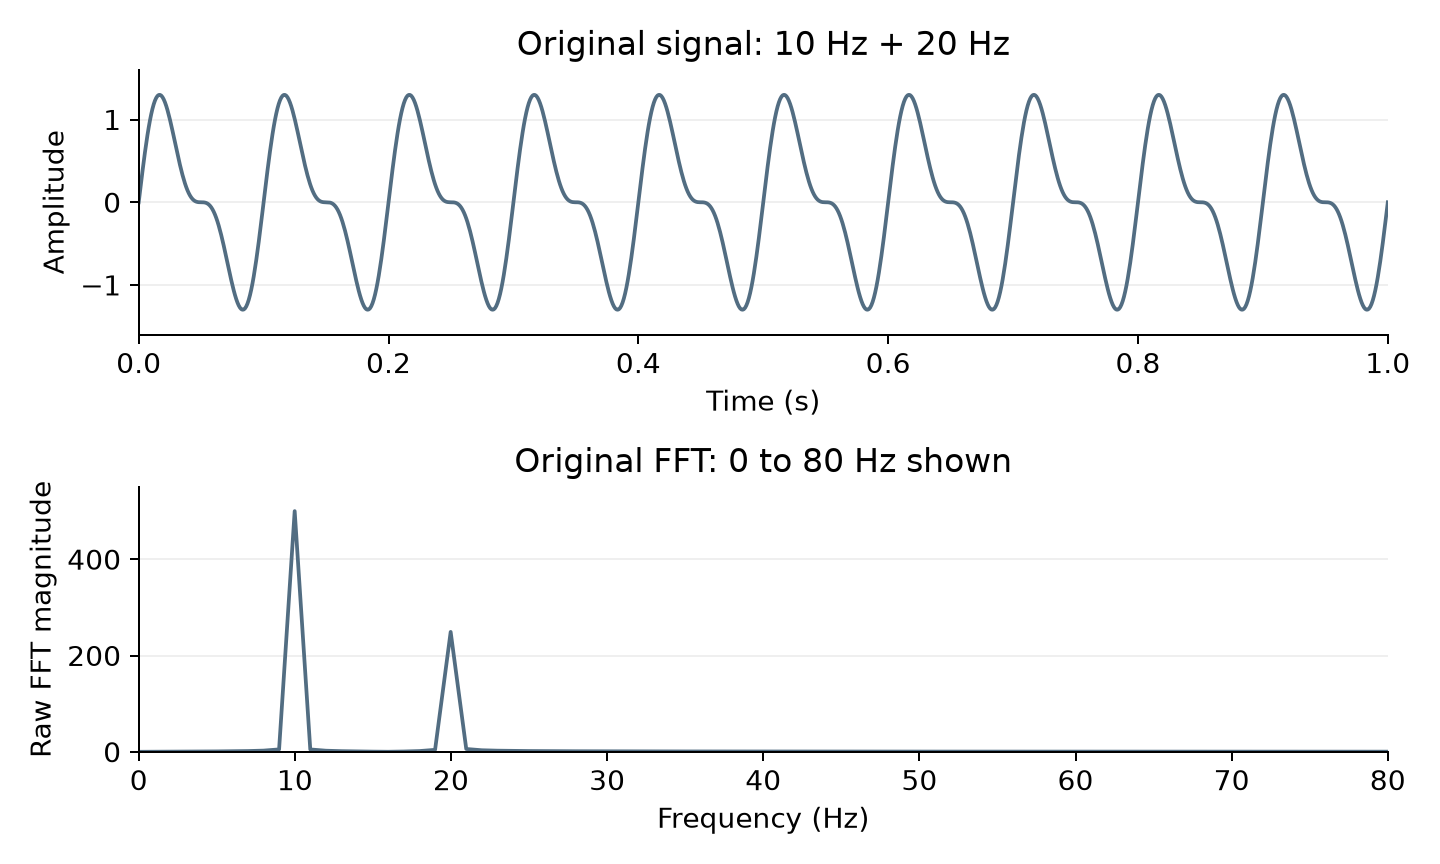
\includegraphics[width=0.92\linewidth]{section1_2_original_fft.png}
\caption{The original two-sine signal and its FFT magnitude. The frequency plot shows 0--80 Hz.}
\label{fig:fourier-original}
\end{figure}

\subsubsection*{Q2. Modify the generate\_signal function to include a 30 Hz component. How does this change the frequency domain representation?}
\textbf{Answer:} A 30 Hz sine with amplitude 0.3 was added.
A new peak appears at 29.97 Hz, with a raw FFT magnitude of 148.72.
The 10 Hz and 20 Hz peaks remain (Figure~\ref{fig:fourier-comparison}).

\subsubsection*{Q3. What happens to the frequency domain plot if you add random noise to the signal? Implement this and explain your observations.}
\textbf{Answer:} Gaussian noise with standard deviation 0.18 and seed 1729 was added to the original signal.
Small, irregular values appear across the spectrum, while the two largest peaks stay at 9.99 and 19.98 Hz.
This happens because the noise contains many frequencies (Figure~\ref{fig:fourier-comparison}).

\begin{figure}[H]
\centering
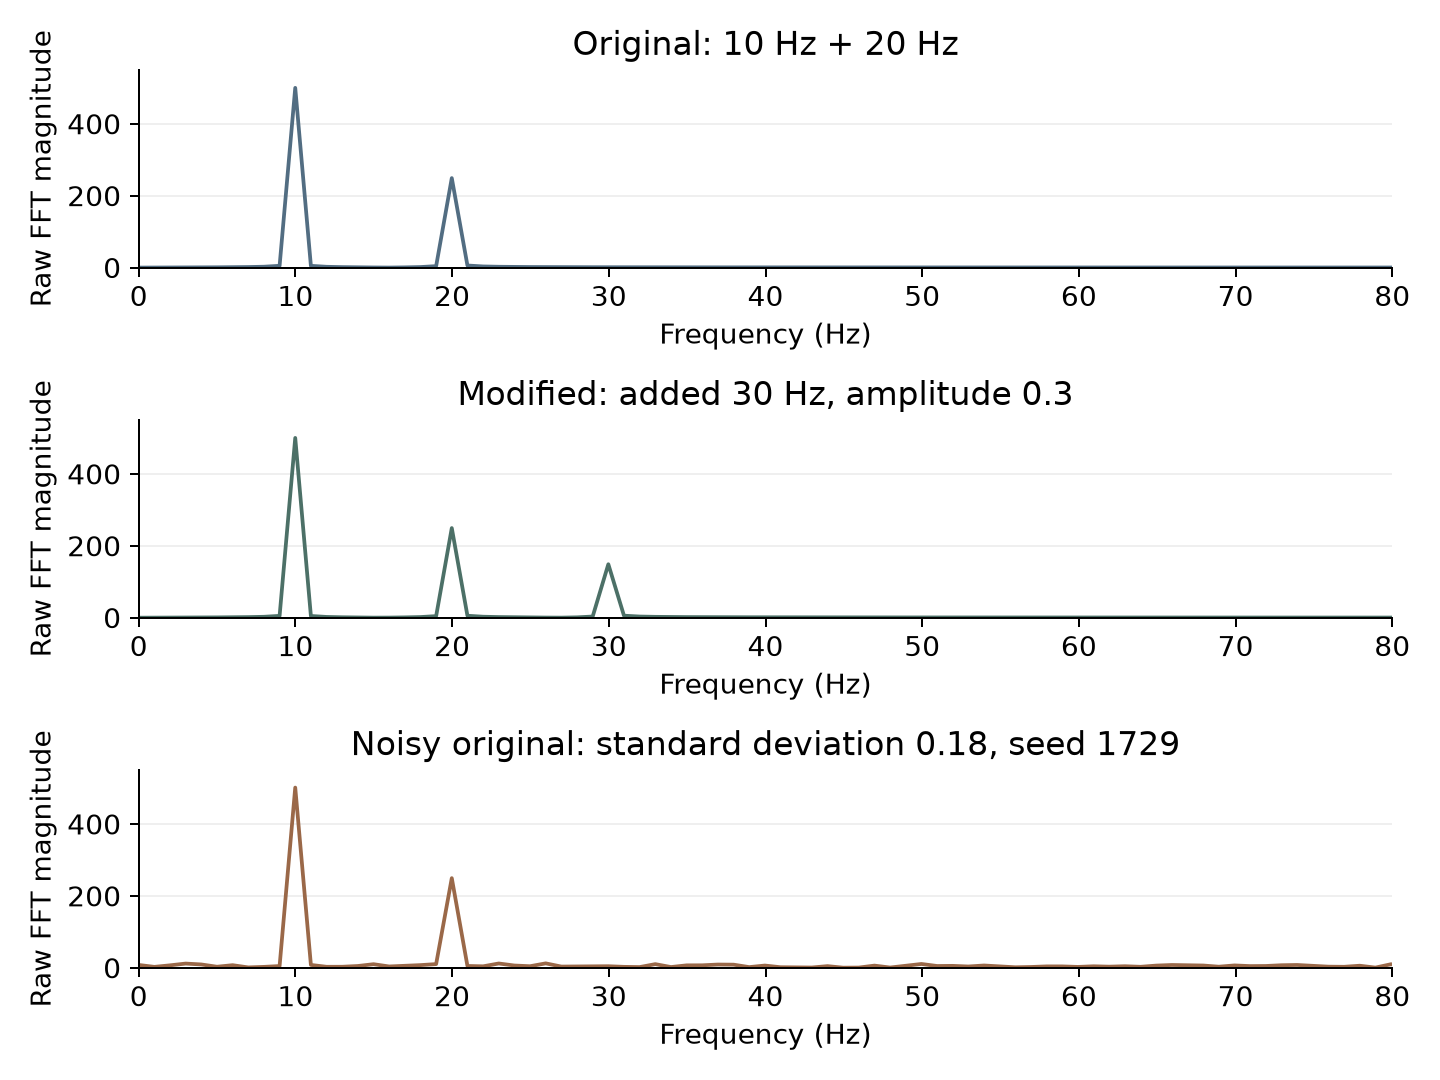
\includegraphics[width=0.92\linewidth]{section1_2_spectra_comparison.png}
\caption{Original, modified and noisy spectra, using the same frequency and magnitude limits. Noise was added to the original signal.}
\label{fig:fourier-comparison}
\end{figure}

\subsubsection*{Q4. Create a function that generates a signal with a frequency that changes over time (e.g., a chirp signal). Plot this signal in both time and frequency domains and explain what you observe.}
\textbf{Answer:} The function sweeps from 15 Hz to 65 Hz in one second.
The waves get closer together over time.
The FFT shows a broad band around this range instead of two narrow peaks.
It shows which frequencies are present, but not when each one occurs (Figure~\ref{fig:fourier-chirp}).

\begin{figure}[H]
\centering
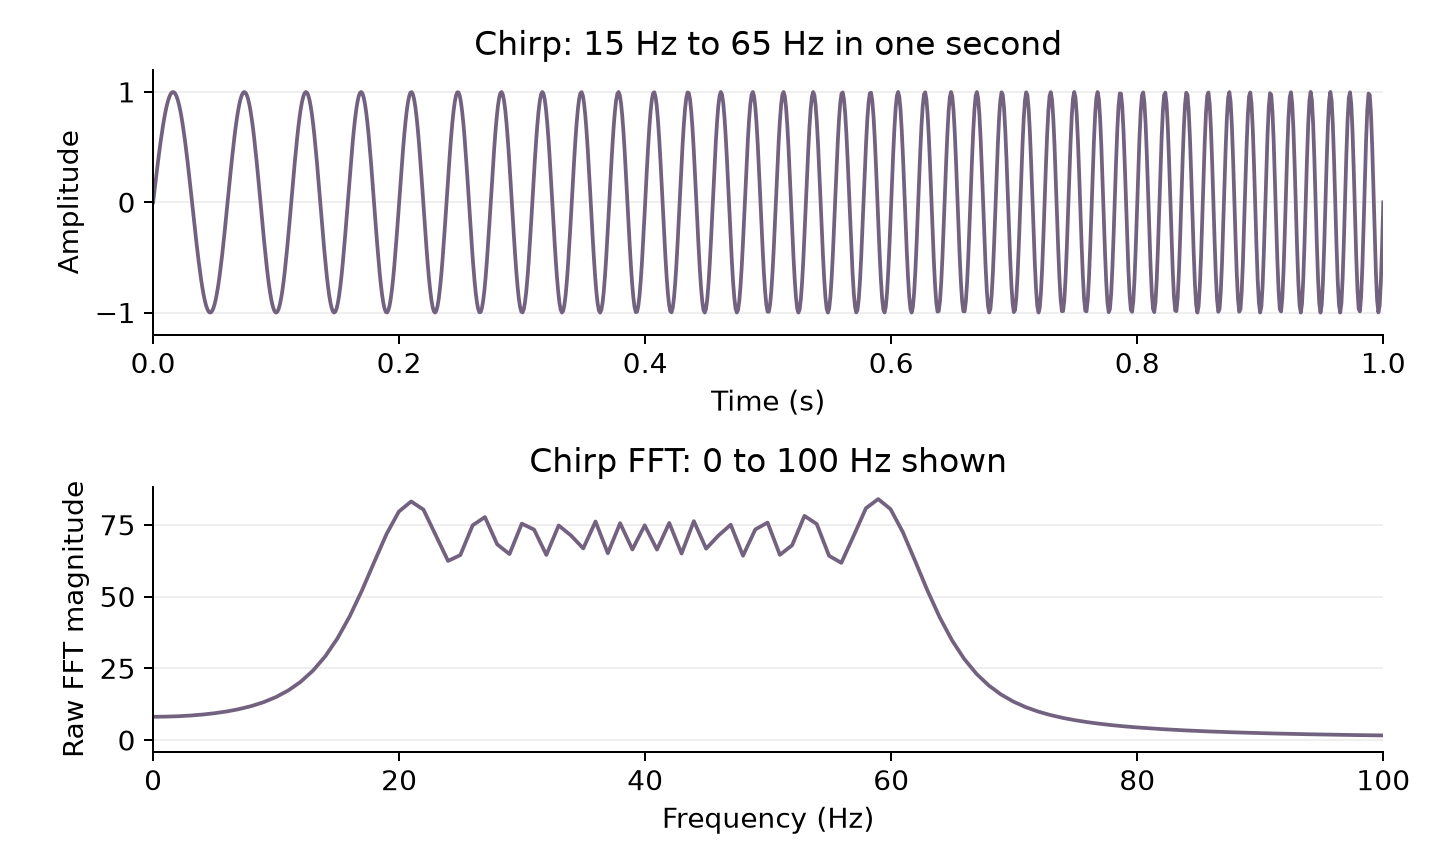
\includegraphics[width=0.92\linewidth]{section1_2_chirp_fft.png}
\caption{The chirp speeds up during the recording. Its FFT magnitude is shown over 0--100 Hz.}
\label{fig:fourier-chirp}
\end{figure}

\subsubsection*{Q5. Describe a practical application where understanding the frequency domain of a signal is important.}
\textbf{Answer:} A sensor can measure a machine's vibration.
Its frequency peaks can be compared with a normal reading.
New or much stronger peaks can help find a fault.

\clearpage
\subsection{Sampling and Aliasing}

\subsubsection*{Q1. What is the Nyquist rate for the given signal? Is the current sampling rate sufficient?}
\textbf{Answer:} For a 10 Hz wave, the Nyquist rate is 20 Hz. The given 15 Hz sampling rate is too low, so the sampled signal shows a false 5 Hz pattern (Figure~\ref{fig:sampling-comparison}).

\subsubsection*{Q2. Increase the sampling rate to 25 Hz. How does this affect the sampled signal's representation of the original signal?}
\textbf{Answer:} I increased the sampling rate to 25 Hz. This is above the 20 Hz Nyquist rate, so there is no aliasing. The extra sample points represent the original 10 Hz wave better (Figure~\ref{fig:sampling-comparison}).

\subsubsection*{Q3. Set the signal frequency to 20 Hz and the sampling rate to 30 Hz. Describe and explain the resulting aliasing effect.}
\textbf{Answer:} I sampled a 20 Hz sine wave at 30 Hz. This is below the required 40 Hz Nyquist rate. The sampled points behave like a \(-10\) Hz sine wave because the sampling rate is too low (Figure~\ref{fig:sampling-comparison}).

\begin{figure}[H]
\centering
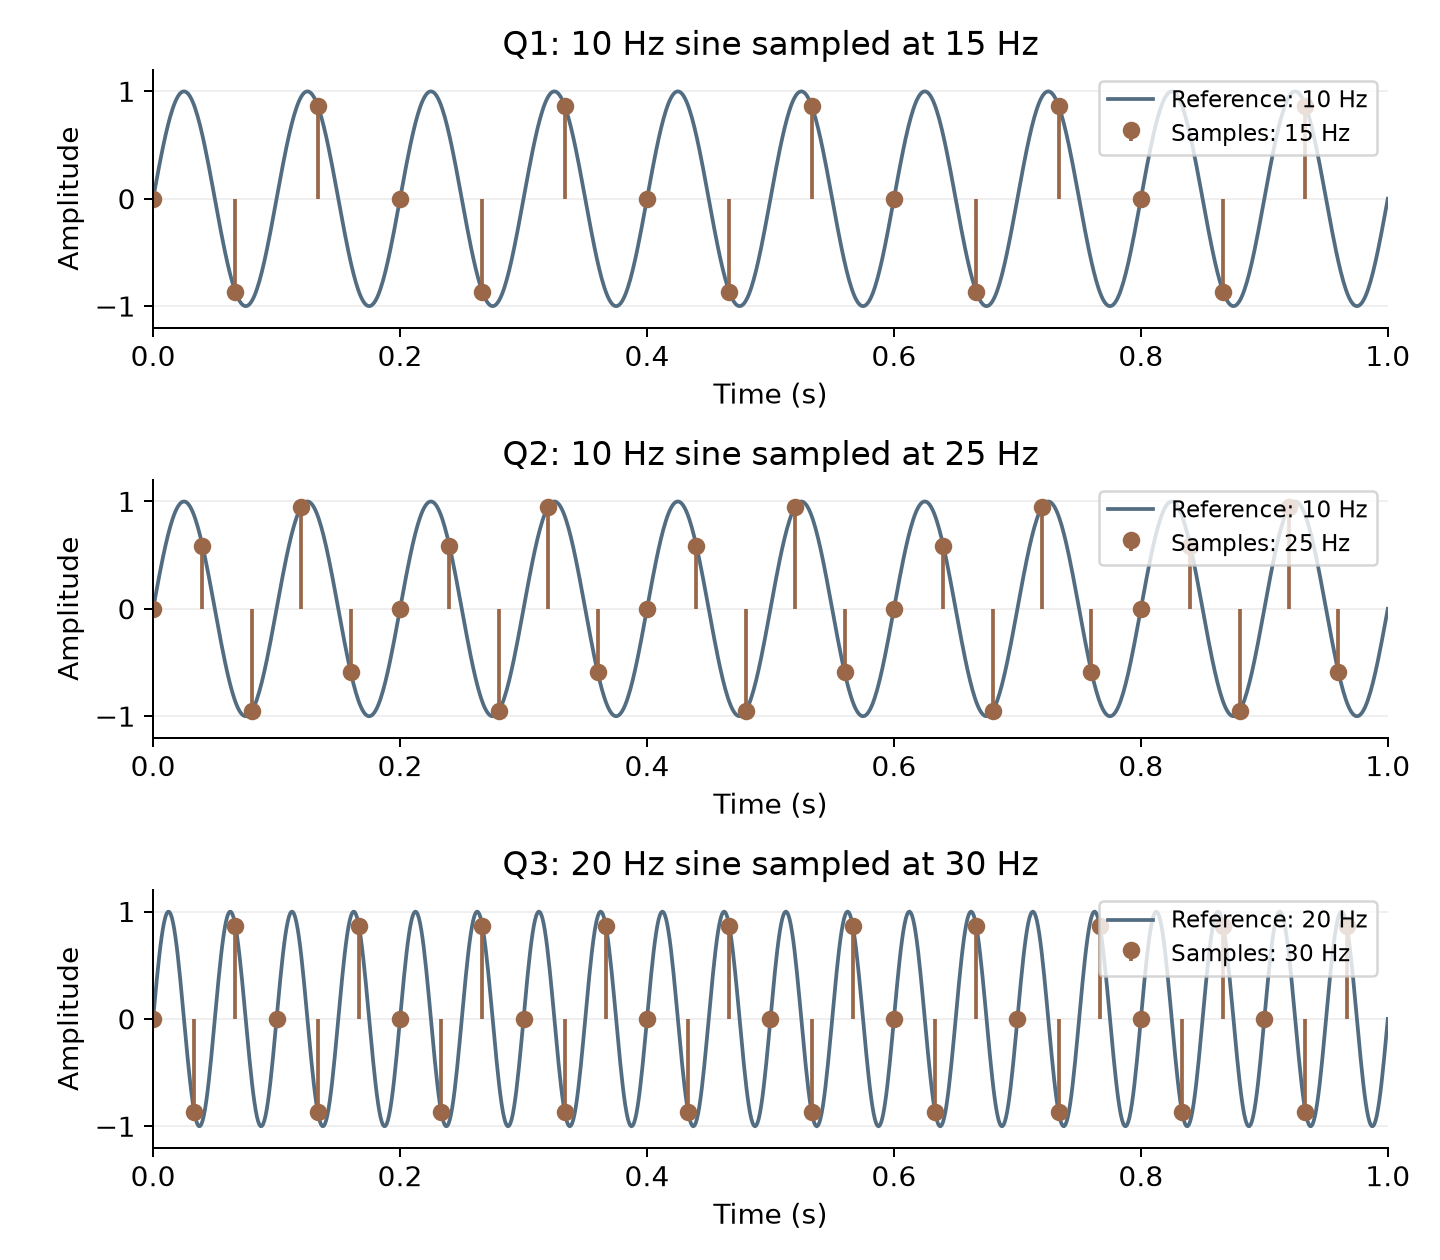
\includegraphics[width=0.92\linewidth]{section1_3_sampling_comparison.png}
\caption{Sampling comparison for the three given cases. The 25 Hz sampling rate represents the 10 Hz signal without aliasing.}
\label{fig:sampling-comparison}
\end{figure}

\subsubsection*{Q4. Create a function that demonstrates the "wagon-wheel effect" by sampling a high-frequency sinusoid at a much lower rate. Plot the original and sampled signals, and explain the visual effect.}
\textbf{Answer:} I sampled a 23 Hz sine wave at 8 Hz. The sampled points match a 1 Hz wave with its sign reversed. This makes a fast repeating signal look much slower, like the wagon-wheel effect (Figure~\ref{fig:wagon-wheel}).

\begin{figure}[H]
\centering
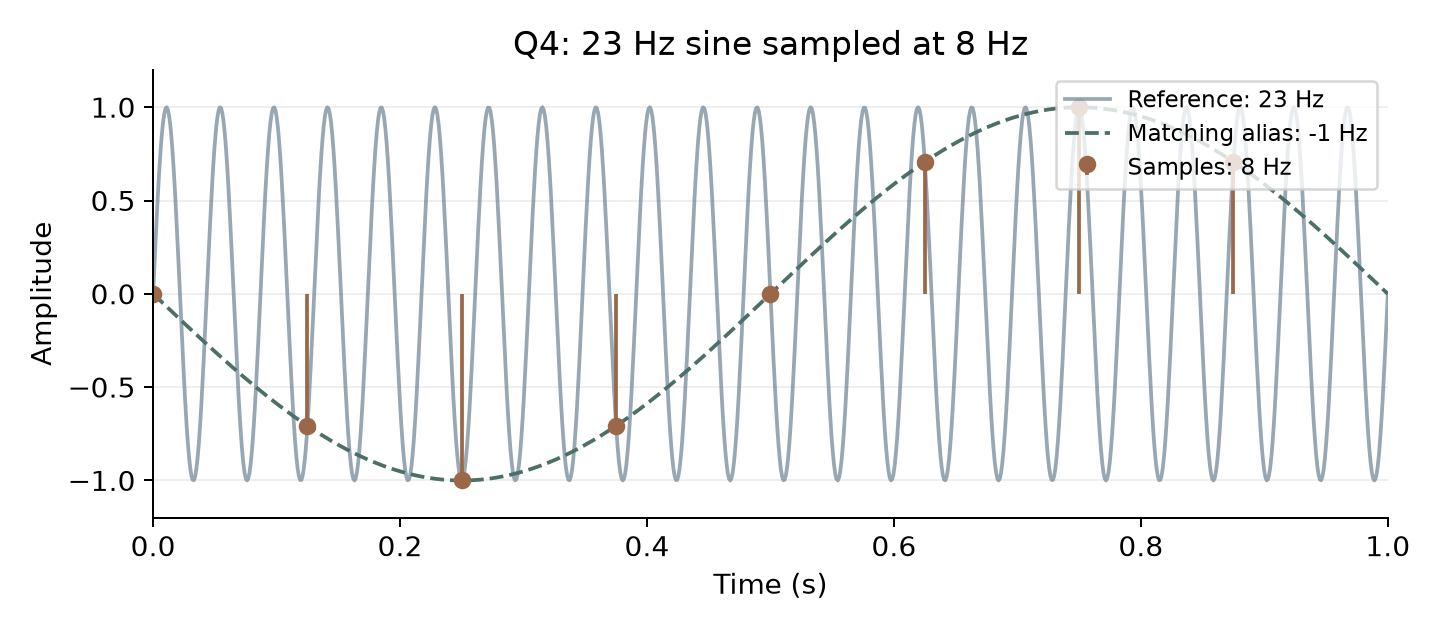
\includegraphics[width=0.92\linewidth]{section1_3_wagon_wheel.png}
\caption{A 23 Hz signal sampled at 8 Hz produces a slow, reversed 1 Hz alias.}
\label{fig:wagon-wheel}
\end{figure}

\subsubsection*{Q5. Describe a real-world scenario where understanding aliasing is crucial.}
\textbf{Answer:} A camera can make spinning fan blades look slower or move backwards when the frame rate is too low. Choosing a high enough frame rate helps show the motion more accurately.

\section{Discussion}
Changing frequency changes the number of cycles, while adding signals changes their shape.
The square-wave comparison also shows why values at zero need to be checked.
With added noise, the main FFT peaks stayed visible above the smaller values.
When the sampling rate was too low, higher frequencies appeared as lower ones.

\section{Conclusion}
The requested signals were generated and compared.
The 20 Hz sine had twice as many cycles, and the composite had both curves and jumps.
Fourier analysis identified the added 30 Hz component and the chirp's wider frequency range.
The sampling experiments showed how aliasing can give a false impression of the original signal.

\section*{Appendix: Code Snippets}
\begin{verbatim}
sawtooth_wave = 2 * (5 * t - np.floor(5 * t)) - 1
square_wave_ceil = np.ceil(np.sin(2 * np.pi * 5 * t)) * 2 - 1
\end{verbatim}
The first line removes whole cycles to make a repeating ramp.
The second line is the teacher's replacement expression checked in Q3.
The full script is \texttt{code/section1\_1.py}.
The Fourier analysis script is \texttt{code/section1\_2.py}.

\smallskip
\textbf{Sources:} DT081A Lab 1 assignment, Sections 1.1--1.2 (pages 1--2),
and the DT081A lab report template.
\end{document}
